\subsection{Overview}
\label{sec:results-overview}

Data analysis was conducted on multiple \glspl{data-view}: \textit{Tweets}, \textit{Users} and \textit{Hashtags}. The difference between them is the way they are aggregated: \textit{Tweets} view is aggregated by \texttt{week}; \textit{Users} are aggregated by \texttt{user\_id}; \textit{Hashtags} are exploded\footnote{The term "explosion" in this context refers to extracting multiple values from a given column into multiple table records such that each value from the column can be uniquely identified by the new table record (row); this process is the opposite of data aggregation} and aggregated by \texttt{hashtags} (content afterward).

Analysis begins by describing what kinds of reactions are happening between Croatian Users on Twitter, and who are the Users driving these reactions. Reactions are categorized into \texttt{Original Tweets}, \texttt{Retweets}, \texttt{Replies} and \texttt{Quotes}. Original Tweets represent all tweets that are not Retweets, Retweets represent tweets shared by other users \textit{without} additional content from the retweeting User to the topic being shared. Quotes represent tweets shared by other users \textit{with} additional content from the quoting User to the topic being shared (a Quote can contain Retweet's content, but a Retweet cannot contain Quote's content), and Replies represent replies to tweets. Additional concepts of \textbf{Incoming links} and \textbf{Outgoing links} (\textbf{reactions}) are introduced (\texttt{Incoming Retweets}, \texttt{Incoming Replies} and \texttt{Incoming Quotes}). An incoming link represents the number of times external users interacted with the User in focus, while an outgoing link represents the number of times the User in focus posted a reaction category.

After the reaction categories are quantitatively described, the content (\texttt{hashtags}) behind those interactions is identified in \ref{sec:results-hashtags}. Once the most popular content is described, outliers ("spam") are detected and filtered to support a resilient qualitative analysis. Graph analysis is introduced to identify and analyse relationships between \textit{Users} and \textit{Hashtags}. Finally, information sharing is visualized as the number of times a \texttt{hashtag} has been shared in a given time range and information spread is visualized as the \texttt{hashtag} percentage share in the total number of Tweets in the collected network.

The analysis is conducted on a total number of \(386,168\) Tweets ranging from \texttt{2022-11-01} to \texttt{2022-11-30}, including \(6,887\) Croatian Users. The total number of Tweets includes \(265,155\) \texttt{Original Tweets} (\(165,719\) \texttt{Replies} and \(24,170\) \texttt{Quotes}) and \(121,013\) \texttt{Retweets}. Incoming links are represented by \(7,034\) \texttt{Incoming Retweets}, \(32,728\) \texttt{Incoming Replies} and \(2,120\) \texttt{Incoming Quotes} (one original Tweet can have multiple incoming links).

\subsection{Tweets}
\label{sec:results-tweets}

The \textit{Tweets} view is aggregated by \texttt{week}, enabling fine data granularity. Figure \ref{figure:tweets-incoming-reactions} shows what reactions are Croatian Users on Twitter mostly engaged with in the weeks of November, 2022.

\begin{center}
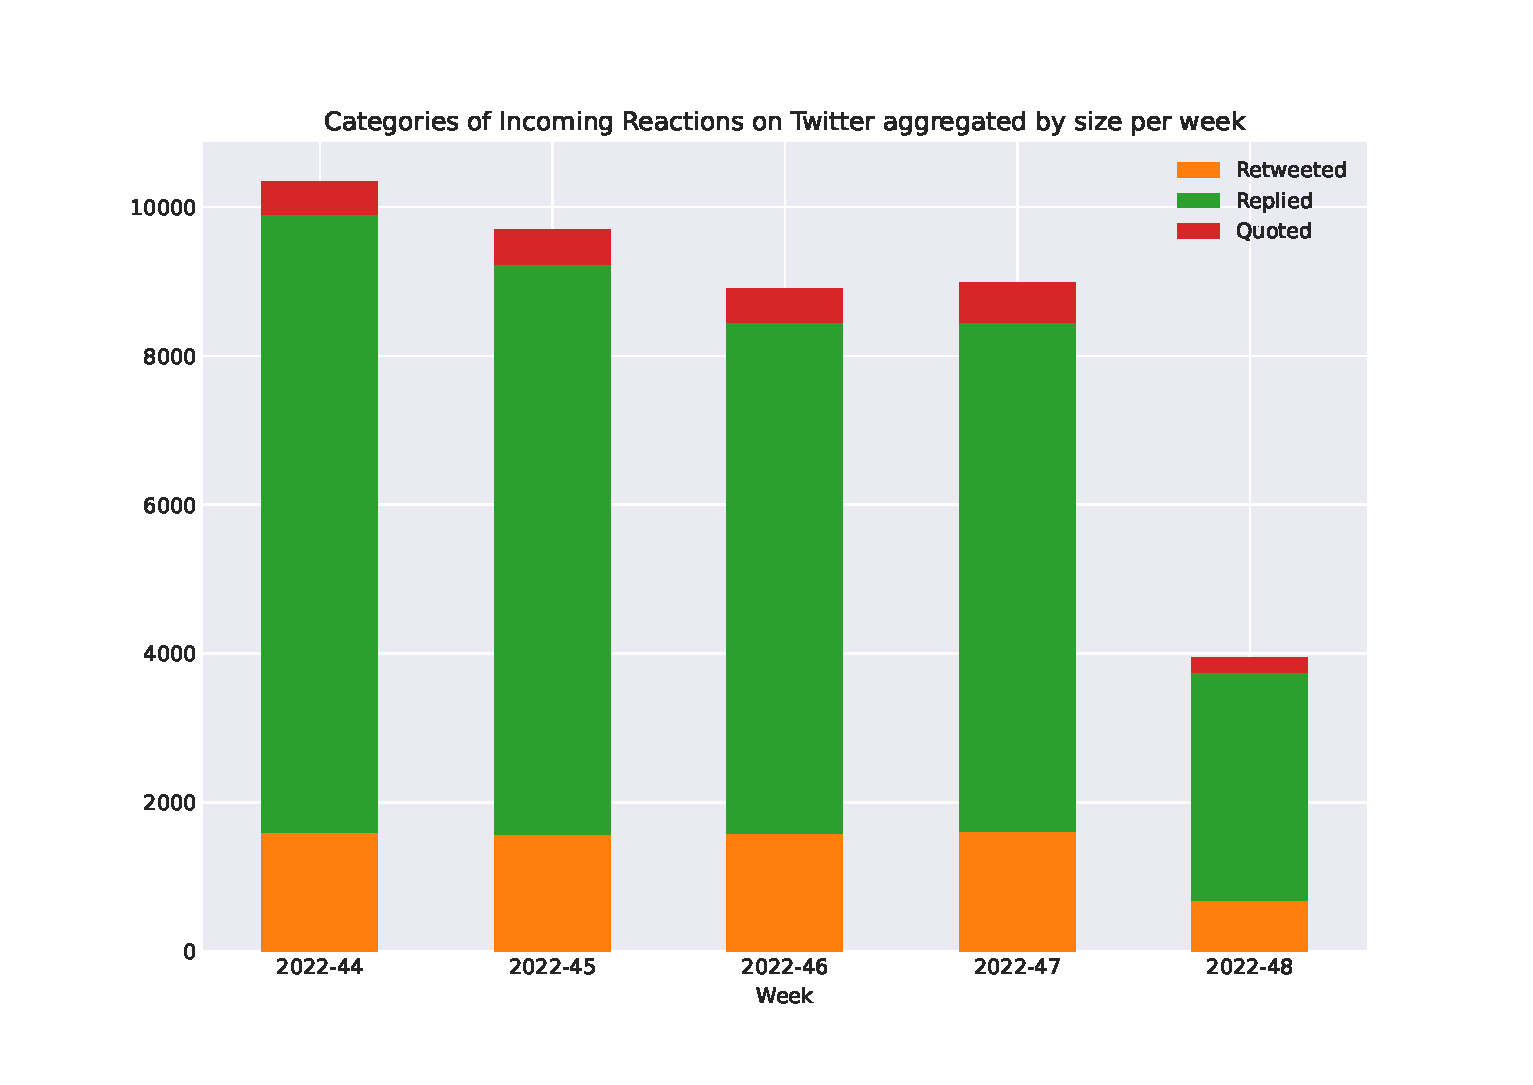
\includegraphics[width=14cm,keepaspectratio]{figures/tweets-incoming-reactions.eps}
\label{figure:tweets-incoming-reactions}
\captionof{figure}{Categories of Incoming Reactions on Twitter aggregated by size per week}
\end{center}

This visualization shows that the largest amount of Users is engaged in \textit{Reply} reactions - however, the \textit{Hashtags} analysis shows that most content is shared using the \textit{Retweet} reactions, disregarding that most incoming reactions are really \textit{Replies}.

\subsection{Users}
\label{sec:results-users}

This view is aggregated by \texttt{user\_id}, disabling a fine time aggregation granularity but enabling a total overview of a User's reactions. All visualizations based on the Users view display the total amount of a User's reactions in the given time range and his collected Tweets. Figure \ref{figure:users-total-in-initiators} shows which Users are the incoming reaction initiators.

\begin{center}
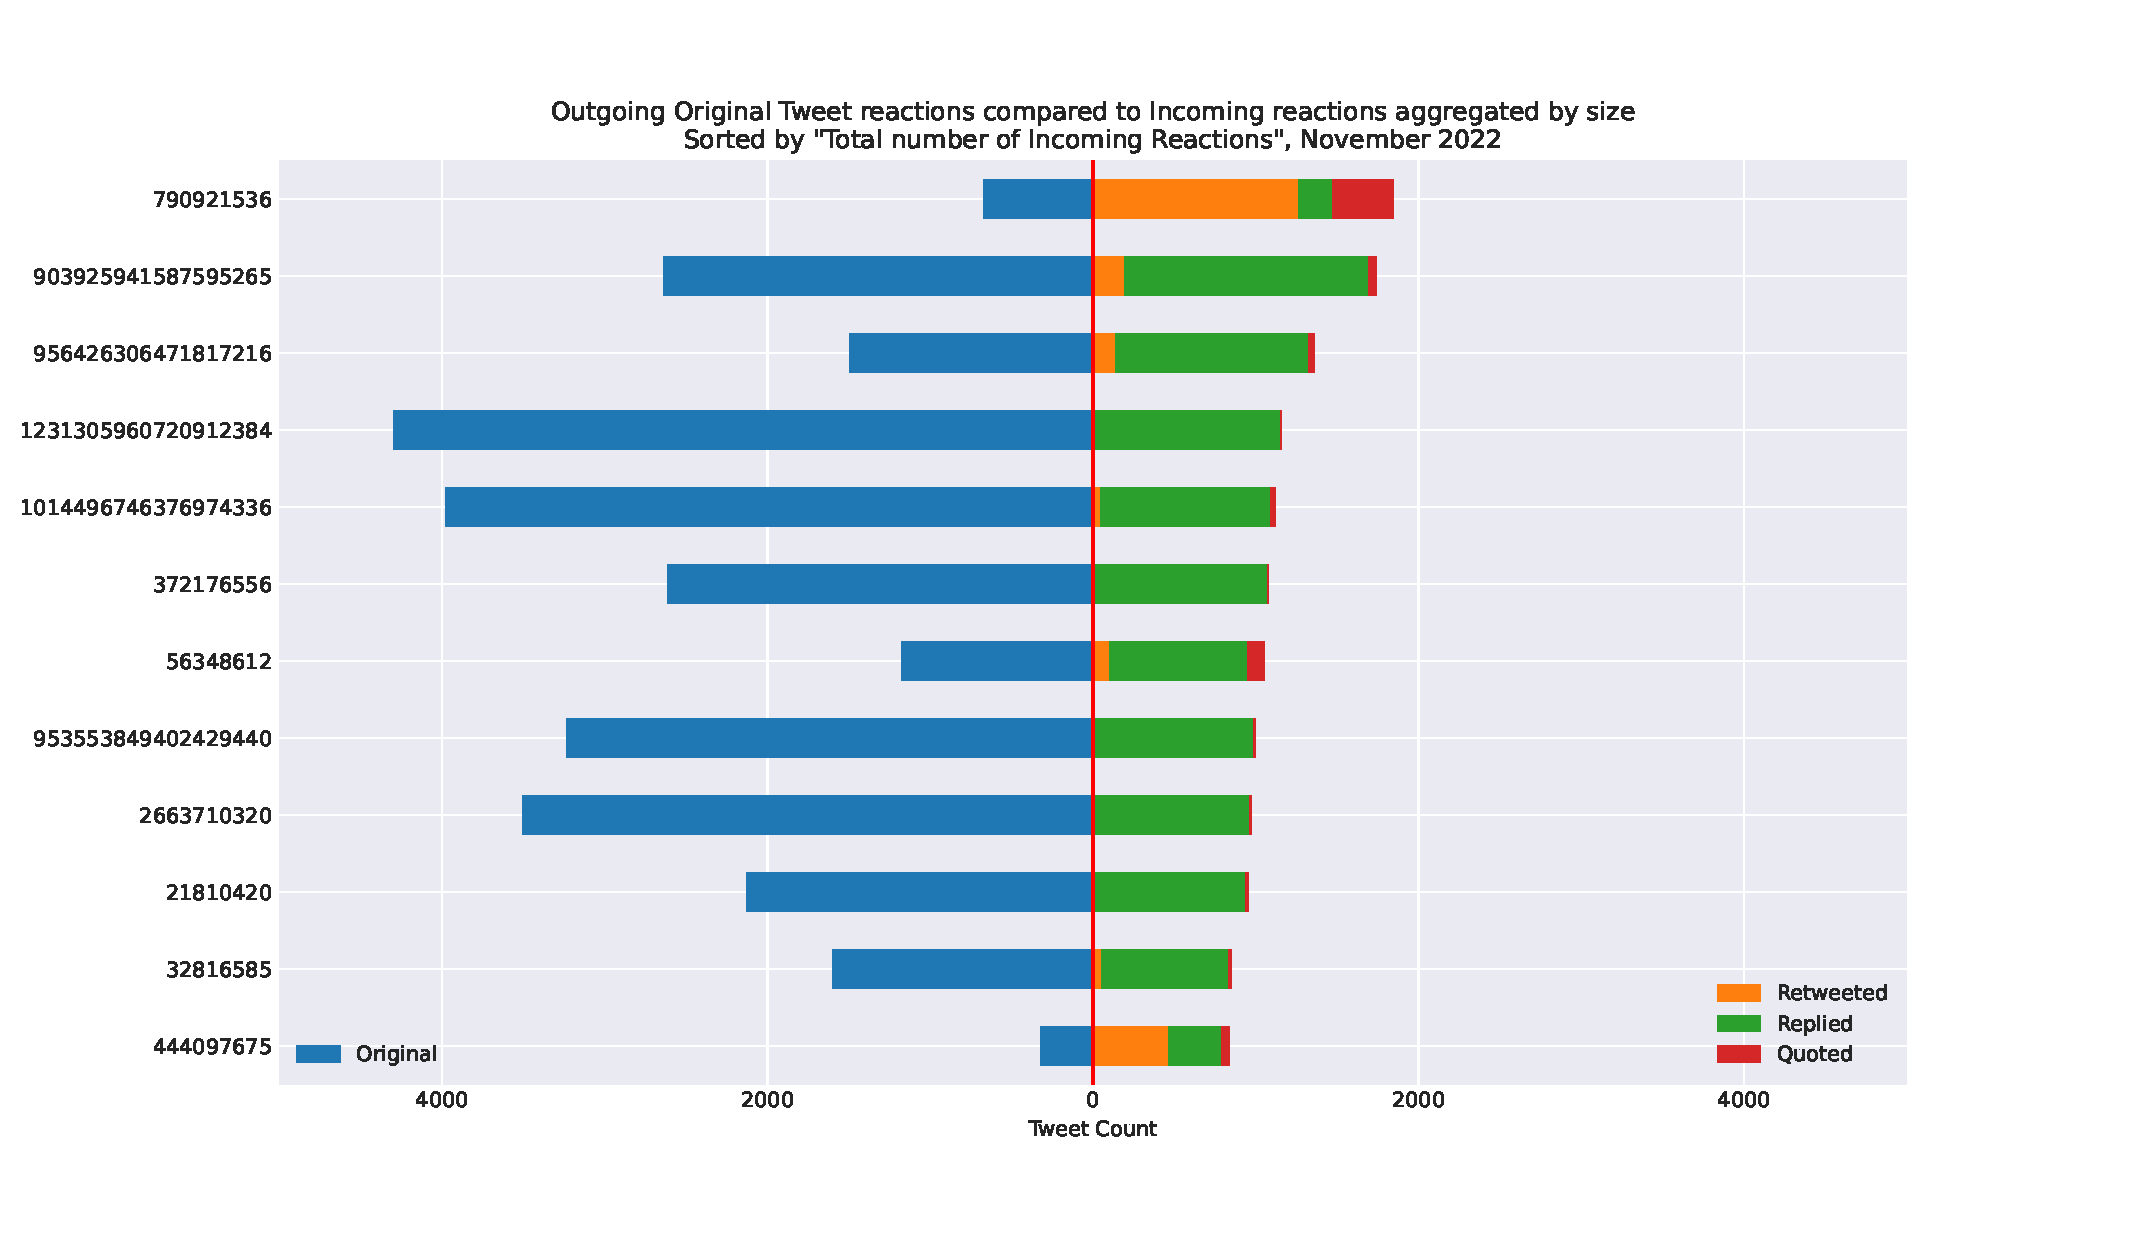
\includegraphics[width=16cm,keepaspectratio]{figures/users-total-in-initiators.eps}
\label{figure:users-total-in-initiators}
\captionof{figure}{Outgoing Original Tweet reactions compared to Incoming reactions aggregated by size}
\end{center}

This visualization shows the categories of reactions that the initiators participate in and it confirms that the largest amount of Users is engaged in \textit{Reply} reactions. See the amount of users engaged in \textit{Retweets} in Appendix \ref{part:appendix}. 

To understand how much users are involved in each reaction categories, figure \ref{figure:users-reaction-distribution} shows the percentage distribution of a User's involvement in \texttt{Outgoing Original Tweets}, \texttt{Incoming Retweets} and \texttt{Incoming Replies}.

\begin{center}
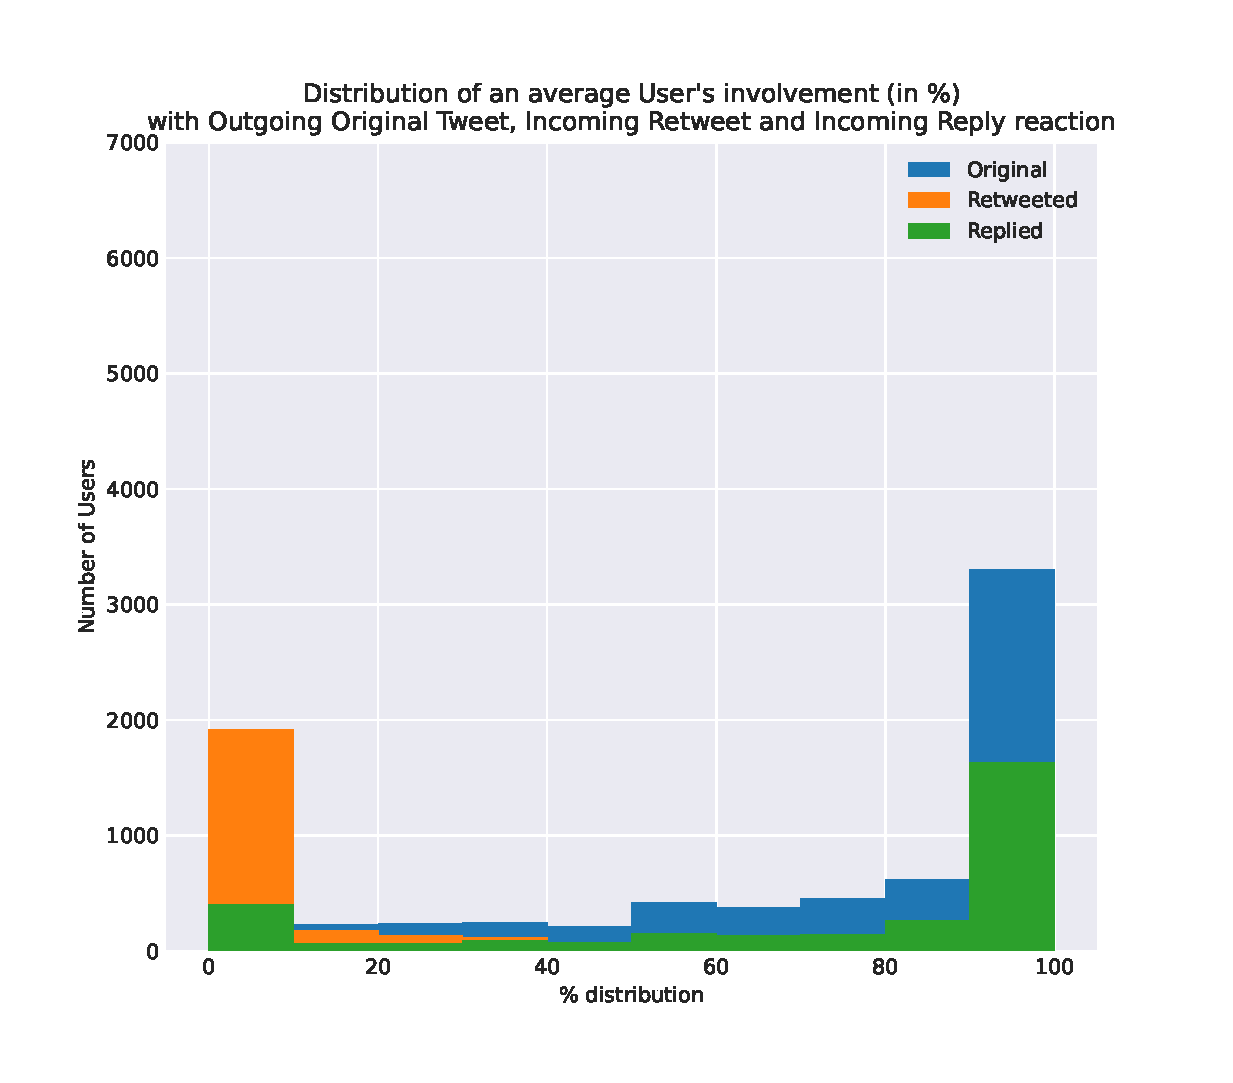
\includegraphics[width=16cm,keepaspectratio]{figures/users-reaction-distribution.eps}
\label{figure:users-reaction-distribution}
\captionof{figure}{Distribution of an average User's involvement (in \%) with Outgoing Original Tweets, Incoming Retweets and Incoming Reply reactions}
\end{center}

This visualization shows how most Users on Twitter mostly tweet \texttt{Original Tweets} and how most Users get replied to (\texttt{Incoming Replies}) (more than \(3,000\) Users). About \(~1,500\) Users' tweets get retweeted (\texttt{Incoming Retweets}), in a very small amount.

\subsection{Hashtags}
\label{sec:results-hashtags}

Previous results have shown what are the reactions on Twitter that Users are most likely to engage with. This section analyses what content is being shared using the described reactions. Figure \ref{figure:hashtags-total-in-reactions} shows what content is being shared the most, sorted by the number of total incoming reactions.

\begin{center}
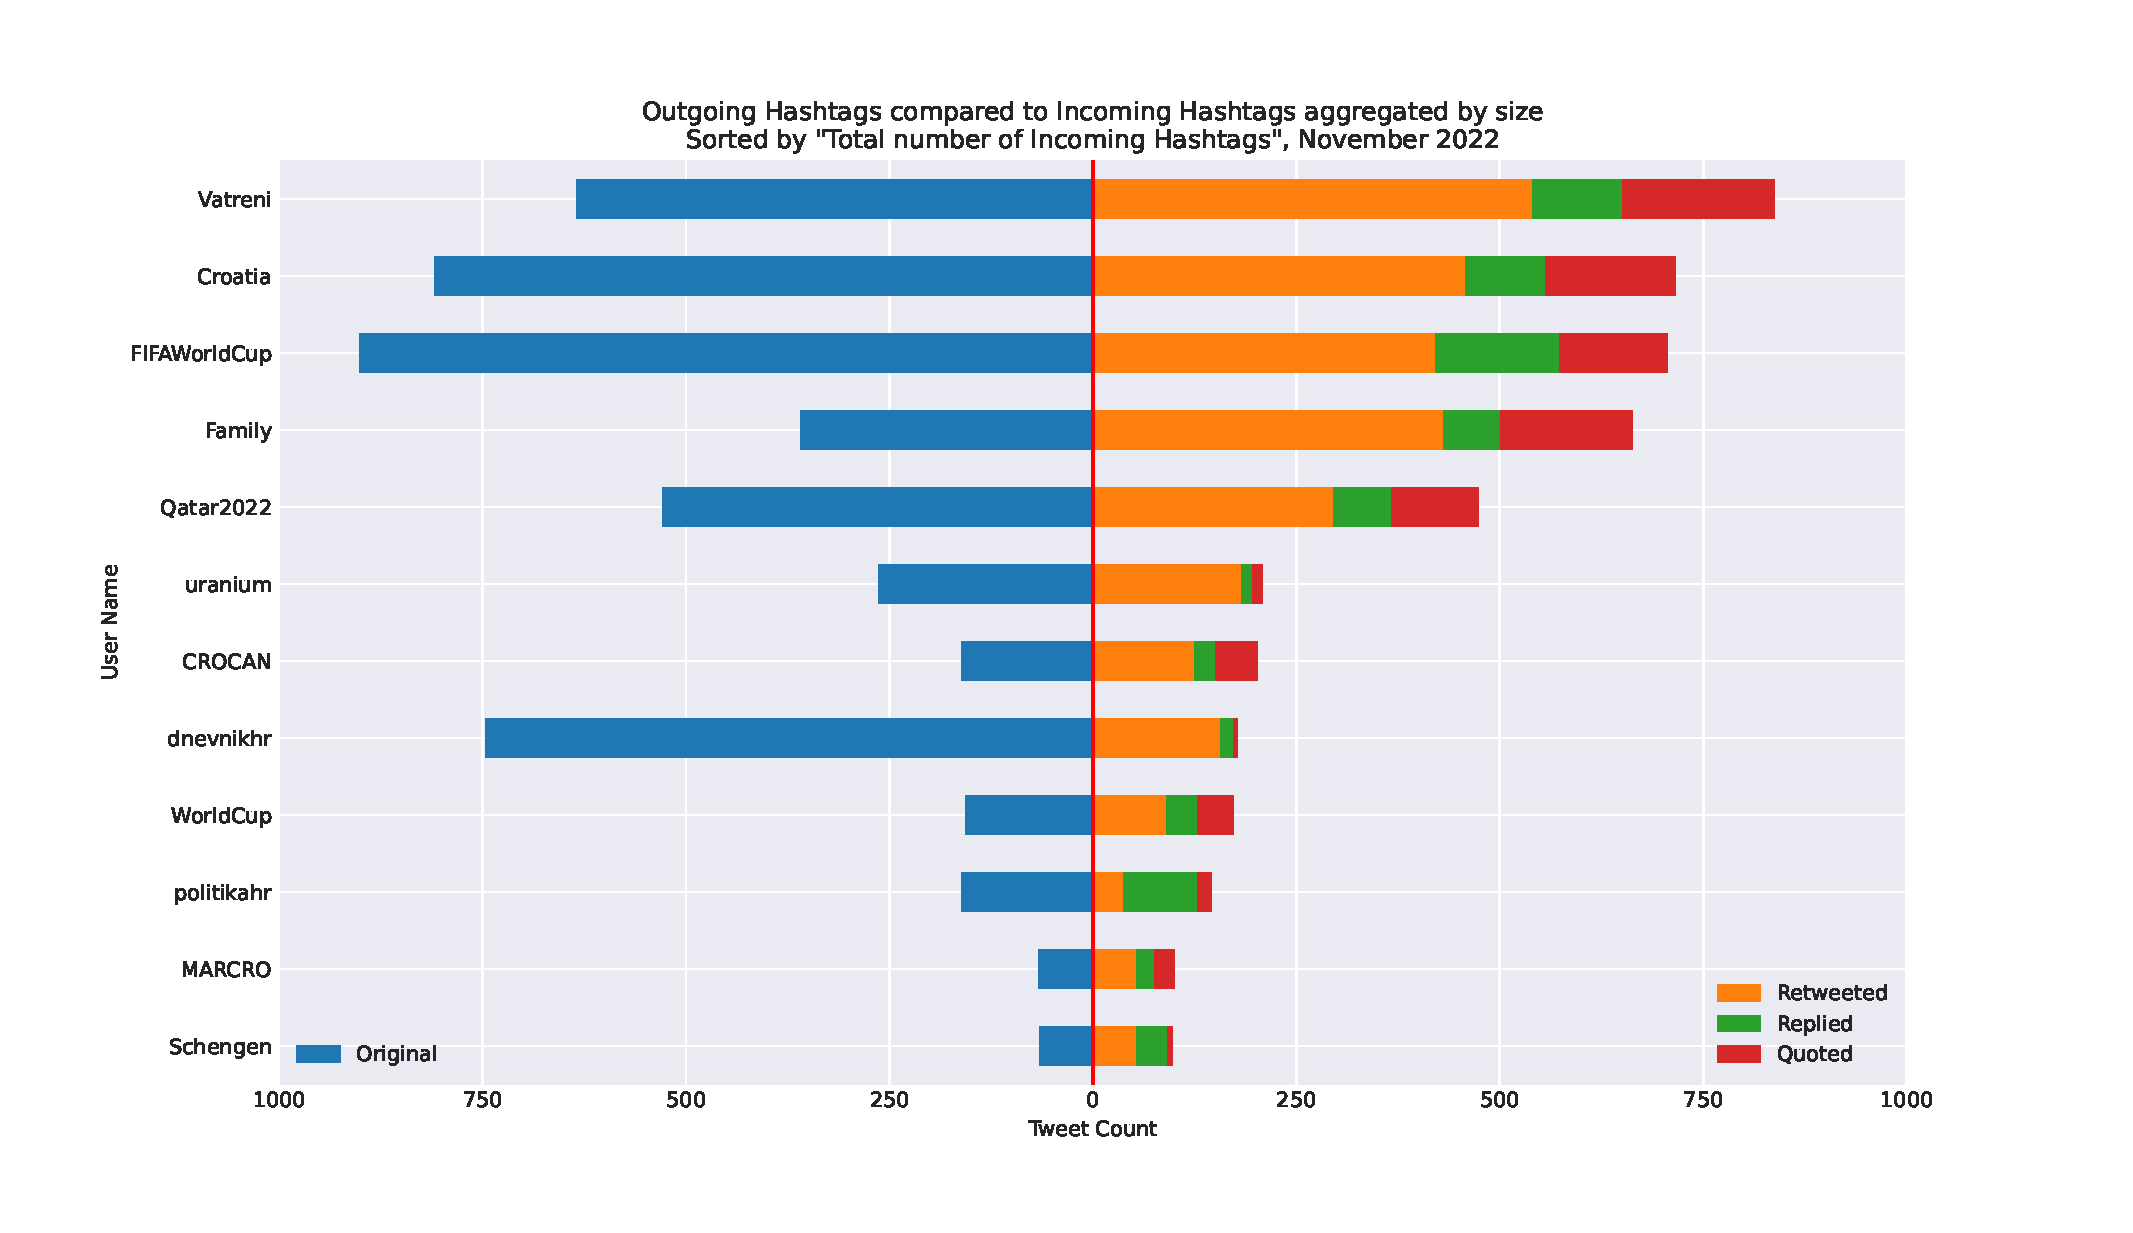
\includegraphics[width=16cm,keepaspectratio]{figures/hashtags-total-in-reactions.eps}
\label{figure:hashtags-total-in-reactions}
\captionof{figure}{Outgoing Hashtags compared to Most Popular Incoming Hashtags aggregated by size}
\end{center}

This visualization confirms that the most popular content is spread using the \textit{Retweet} reaction. The spread of the most popularly shared content, \texttt{Vatreni} hashtag, is related to the FIFA World Cup which is taking place in the analysed time span. It is important to note that this analysis is short-sighted because of the short time span it covers. More visualizations on reaction categories are available in Appendix \ref{part:appendix}.

While performing this analysis, some content was identified as "spam", i.e. there is a specific group of Users who continuously share the same content, without external users sharing that same content. This behavior causes a quantitative bias where some content appears to have a large number of incoming reactions, even though they are all coming from the same User and are not being shared across the network. To identify such biases, additional data features are introduced - \(\alpha\) (\texttt{alpha}) and \(\beta\) (\texttt{beta}). 

\(\alpha\) and \(\beta\) are calculated using the unique number of Users who at least once shared the hashtag, and the total number of times that the hashtag was shared. The collected data is referenced as \(D\), Users are referenced as \(u\in D_u\), and Hashtags are referenced as \(h\in D_h\):

\[
 HU = \{(h, u) \mid h \in D, u \in D\}
\]
\[
 w(h) \colon= \#{i\colon(h, i) \mid h \in HU}
\]
\[
 w(hu) \colon= \#{i\colon(h, u, i) \mid (h, u) \in HU}
\]

\[
 \alpha = \{w(hu) / w(h) \mid (h, u)\in HU, h\in D_h\}
\]
\[
 \beta = \{w(hu) / \sum_{i=0}^{\lvert D_h\lvert} w(h) \mid (h, u)\in HU, h\in D_h\}
\]

Finally, \(\alpha\) and \(\beta\)are normalized.

\[
 \alpha = \{a\colon \alpha * (1 / max(\alpha)) \mid a\in \mathbb{R}, a\geq 0.0, a\leq 1.0\}
\]
\[
 \beta = \{b\colon \beta * (1 / max(\beta)) \mid b\in \mathbb{R}, b\geq 0.0, b\leq 1.0\}
\]


Figure \ref{figure:hashtags-popularity} displays \(\alpha\) as the normalized number of unique Users who shared the content, \(\beta\) as the normalized ratio a content has in the entire set of available contents. Popular content that is shared among a large number of users has a high \(\alpha\), while content shared among a small number of Users has a low \(\alpha\). Popular content that is included in the majority of the content being shared has a high \(\beta\), while content that is included in the minority of the content being shared has a low \(\beta\). 

\begin{center}
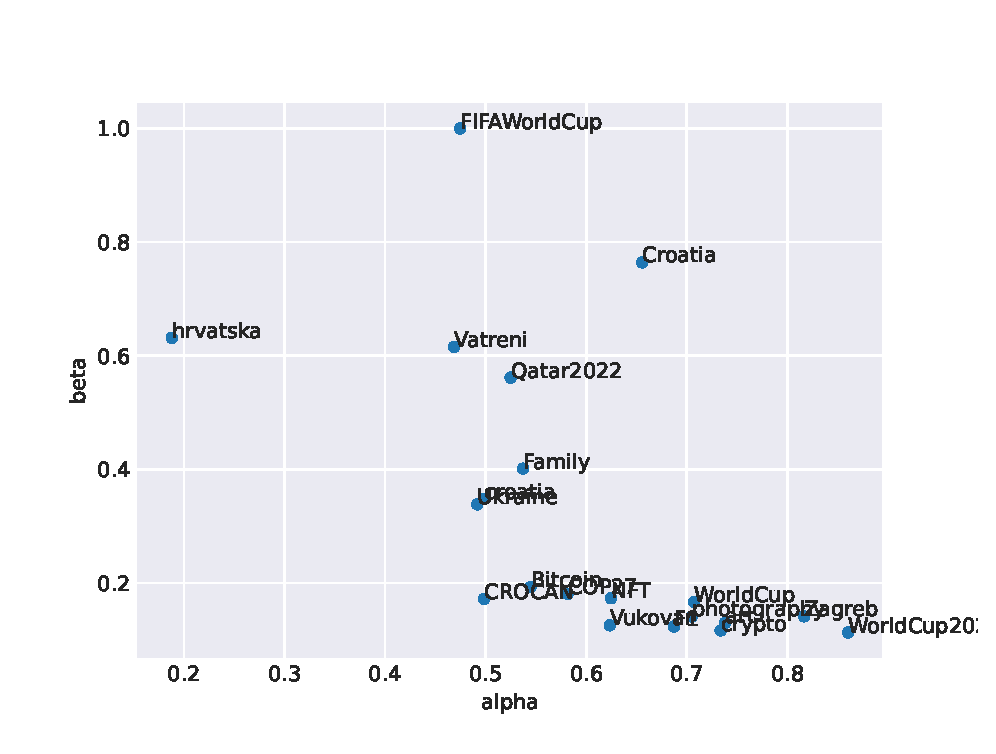
\includegraphics[width=16cm,keepaspectratio]{figures/hashtags-popularity.eps}
\label{figure:hashtags-popularity}
\captionof{figure}{Hashtag Popularity based on the derived \(alpha\) and \(beta\) (normalized) features}
\end{center}

This figure shows that the content \texttt{Vatreni} is shared among \(~ 50\%\) of users and it is included in \(~ 60\%\) of the content being shared. On the other hand, contents \texttt{WorldCup} and \texttt{photography} are shared among \(~ 75\%\) of users, but it is included only in \(< 20\%\) of the content being shared.

At the time of writing this thesis, an automated process of topic detection is not implemented, so topics are manually derived using the observations from preceding figures, and defined as: "World Cup", "Ukraine/War", "Schengen" and a minority of others such as "Crypto" or "SpotifyWrapped" topics. These topics can now be fine-grained by their related content, that is \texttt{FIFAWorldCup}, \texttt{CROCAN}, \texttt{MARCRO}, \texttt{Vatreni} and similar for "World Cup", \texttt{Ukraine} for "Ukraine/War" and so forth. The content is additionally fine-grained by "day" and "week". Figure \ref{figure:hashtags-evolution-daily-202211} shows the number of hashtag occurrences per day in November, 2022.

\begin{center}
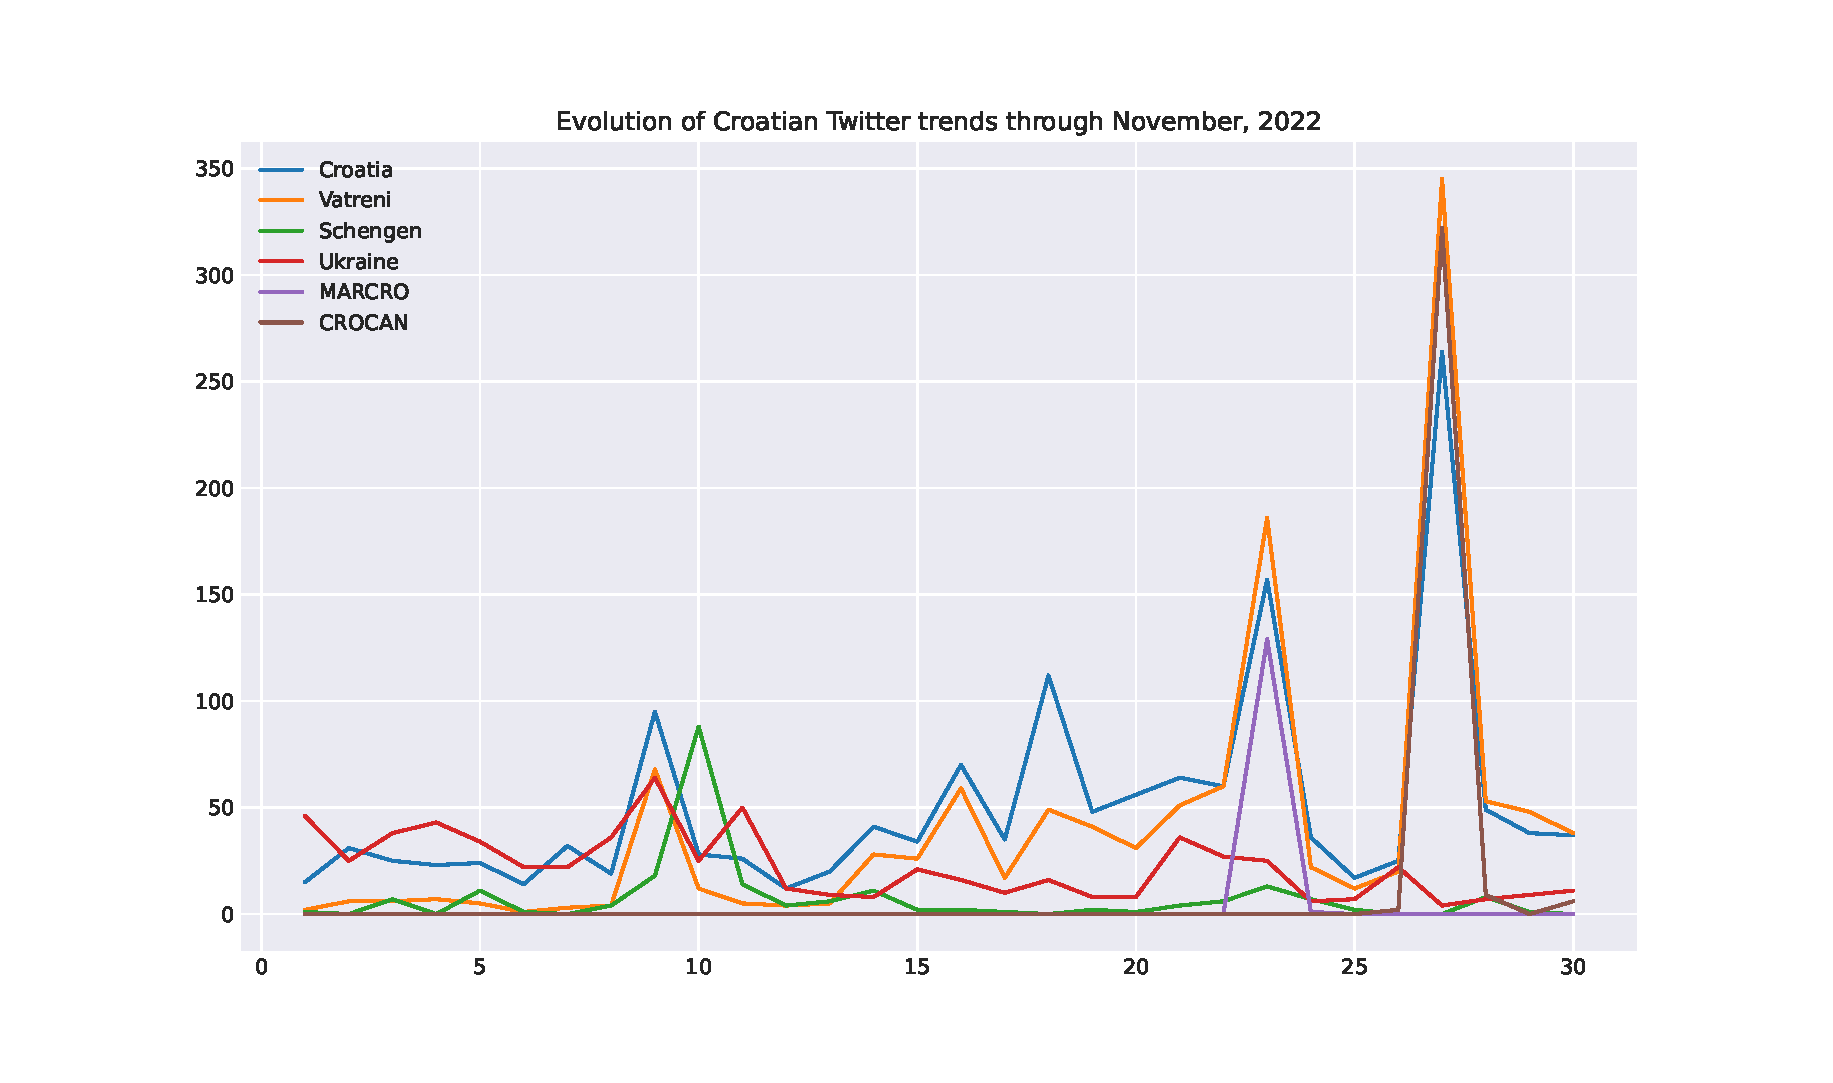
\includegraphics[width=16cm,keepaspectratio]{figures/hashtags-evolution-daily-202211.eps}
\label{figure:hashtags-evolution-daily-202211}
\captionof{figure}{Evolution of Croatian Twitter trends through days in November, 2022}
\end{center}

This figure shows certain hashtag spikes on specific days, like the spike of \texttt{Ukraine} content happening on November 9\textsuperscript{th}, when Russia backed out their troops from Kherson and the EU offered a significant financial support for Ukraine in 2023\cite{euronews2022ukraine}, the spike of \texttt{Schengen} and \texttt{Croatia} content happening on November 10\textsuperscript{th} when Croatia's Schengen request was approved\cite{reuters2022croschengen}, and the spike of \texttt{Vatreni}, \texttt{MARCRO} and \texttt{CROCAN} content happening at the time with World Cup matches between Morocco and Canada versus Croatia (November 23\textsuperscript{rd}, November 27\textsuperscript{th} respectively). Additional analysis on content changing through time is not created as a part of this thesis.

\clearpage
\subsection{Graph Analysis}
\label{sec:results-graphs}

Previous sections provided insights into the contents' quantity and ways that they are shared throughout the network. This sections aims to provide an insight into the relationship between \textit{Users} and \textit{Hashtags}, and finally about the way content is spread throughout the network.

In the following network, a directed graph is presented with \textit{nodes} representing Users who tweet specific content by \textit{edges} where an edge (\(user_i\), \(user_j\)) is represented by an arrow, pointing from the User whose tweet was Retweeted to the User who Retweeted the original tweet (an \textbf{inverse} Incoming link). Greater arrow thickness represents greater number of Retweets between \(user_i\) and \(user_j\). The nodes are colored by their clustering coefficient, which is discussed later in this section.

The number of available tweets in the network increases every day, while the analysis created as a part of this thesis only displays information from a fixed time range. By running this same analysis on a dataset in a different time range, the results could change dramatically. This effect makes this network a \textbf{\gls{temporal-network}}, also known as a \textbf{time-varying network}.

Figure \ref{image:graph-topic-Vatreni} shows the spread of the \texttt{Vatreni} content. The node that was Retweeted the most (most Incoming links) is positioned in the center of the graph, it represents the mainstream medium.

\begin{center}
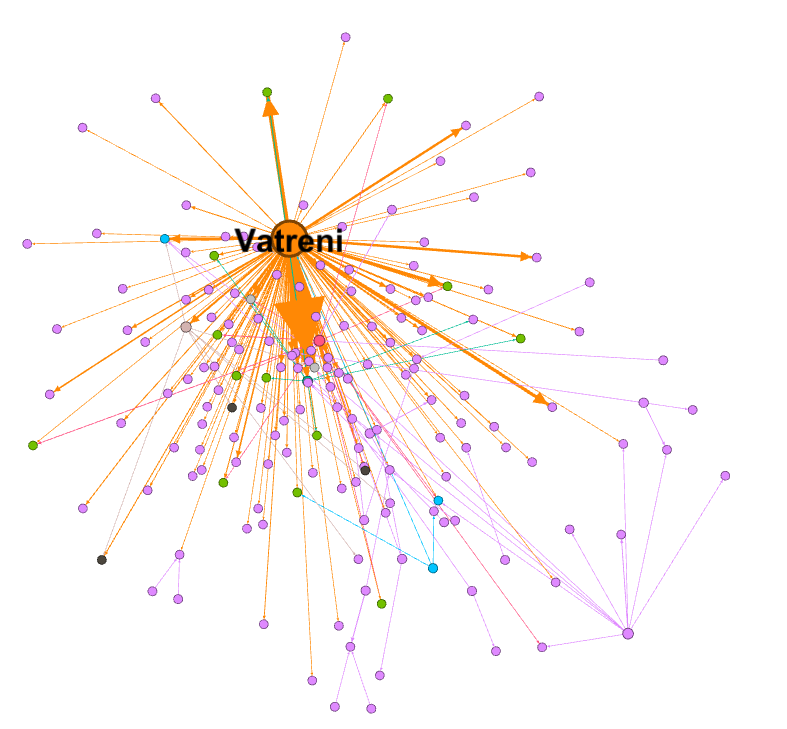
\includegraphics[width=16cm,keepaspectratio]{images/graph-topic-Vatreni.png}
\label{image:graph-topic-Vatreni}
\captionof{figure}{Hashtag Spread across all Users who retweeted Vatreni}
\end{center}

\clearpage
Figure \ref{image:graph-topic-crypto} shows the spread of \texttt{crypto} content. The center of the graph is a node that was retweeting the most (most inverse Outgoing links), the leaflet distributor.

\begin{center}
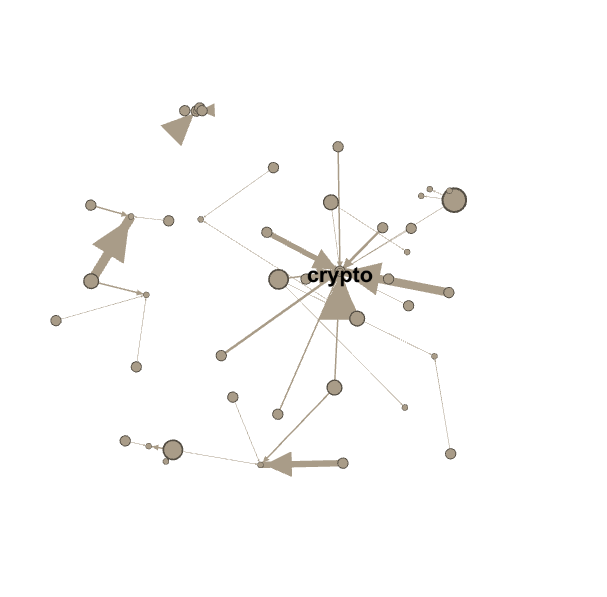
\includegraphics[width=16cm,keepaspectratio]{images/graph-topic-crypto.png}
\label{image:graph-topic-crypto}
\captionof{figure}{Hashtag Spread across all Users who retweeted crypto}
\end{center}

The main differences between these two graphs are their in and out-degrees and their clustering coefficients. \texttt{Vatreni} content was shared by a lot of Users who would usually retweet it from the same User. The User tweeting \texttt{Vatreni} has a high in-degree and low out-degree with a high clustering coefficient that positions the User in the middle of the displayed cluster of nodes. In contrast, \texttt{crypto} content was shared by a small number of Users from different sources. The Users tweeting \texttt{crypto} have a low in-degree and high out-degree with a low clustering coefficient. This pattern is explored using a correlation matrix.

The correlation matrix in figure \ref{figure:graph-measures-correlation} shows correlations between graph measures filtered by \texttt{FIFAWorldCup}, \texttt{Vatreni}, \texttt{Croatia}, \texttt{Ukraine}, \texttt{Schengen} and \texttt{CPO27} (subgraphs representing Retweets between Users who tweeted the selected hashtags). Prior to plotting the matrix, an additional feature \textit{popular} was added to the matrix representing the popularity of a hashtag by a boolean variable. Content \texttt{FIFAWorldCup}, \texttt{Vatreni} and \texttt{Croatia} is labeled "popular", while \texttt{Ukraine}, \texttt{Schengen} and \texttt{CPO27} are labeled "not popular". Label definitions are inspired by the differences identified between figures \textit{Vatreni} \ref{image:graph-topic-Vatreni} and \textit{crypto} \ref{image:graph-topic-crypto}.

\begin{center}
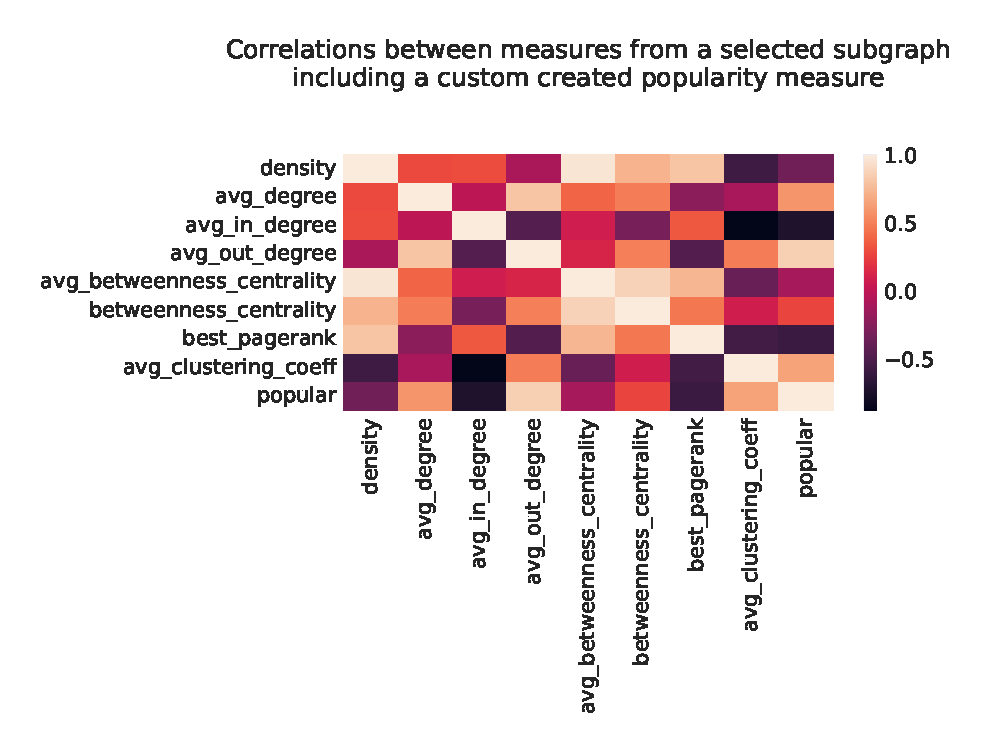
\includegraphics[width=13cm,keepaspectratio]{figures/graph-measures-correlation.eps}
\label{figure:graph-measures-correlation}
\captionof{figure}{Correlations between measures describing selected subgraphs that represent "popular" or "not popular" content}
\end{center}

Following features share the most extreme correlations with the \textit{popular} feature: \textit{avg\_out\_degree} (average Incoming number of links; \(85.34\%\) correlation), \textit{avg\_clustering\_coeff} (average clustering coefficient; \(65.07\%\) correlation) and \textit{avg\_degree} (average Incoming and Outgoing number of links; \(59.35\%\) correlation). These features attribute to the \textit{popular} feature's positivity. On the other hand, features \textit{avg\_in\_degree} (average Outgoing number of links; \(-73.43\%\) correlation) and \textit{best\_pagerank} (node "importance"; \(-59.65\%\) correlation) attribute to the \textit{popular} feature's negativity.

The entire correlation matrix is available in Appendix \ref{part:appendix}.
